% Chapter 1

\chapter{Fachliches Umfeld} % Chapter title

\label{ch:fachlichesUmfeld} % For referencing the chapter elsewhere, use \autoref{ch:introduction}

%----------------------------------------------------------------------------------------
\section{Patentspezifische Begriffe}
\label{ch:fachlichesUmfeld:PatentspezifischeBegriffe}

Um die Motivation für ein Patentinformationssystem, bzw. für den Erwerb der
Dienstleistung DEPAROM-Profil zu verstehen, möchte ich zunächst einige
Fachbegriffe aus dem Bereich Patente/Schutzrecht beschreiben.

\subsection{Patent}
\label{ch:fachlichesUmfeld:PatentspezifischeBegriffe:Patent}

Ein Patent ist eine Art gesellschaftlicher Vertrag, durch den man rechtlichen
Schutz für eine Erfindung erhalten kann. Durch das Patent erlangt der Erfinder
das alleinige Nutzungsrecht für seine Innovation über einen gewissen Zeitraum,
in Deutschland bspw. über 20 Jahre. \cite{patent} Im Gegenzug muss die Erfindung
aber in Form der Patentschrift für die Allgemeinheit zugänglich gemacht werden.
Patente sollen der Innovationsförderung dienen, in dem Sie sowohl dem Erfinder,
als auch der Allgemeinheit Vorteile verschaffen.

\subsection{Patentüberwachung}
\label{ch:fachlichesUmfeld:PatentspezifischeBegriffe:Patentueberwachung}

Die Patentüberwachung beschreibt den Vorgang, die von den Patentämtern
veröffentlichten Patentschriften nach bestimmten Kriterien zu durchsuchen, und
die für eine Person oder ein Unternehmen relevanten Patentdokumente für eine
weitere Analyse zu sammeln. Diese Kriterien umfassen gewöhnlich den Anmelder des
Patents, den Erfinder, den Technologiebereich (in Form der
Patentklassifizierung), sowie Stichworte aus dem Titel oder der Zusammenfassung
des Patents.

\subsection{Motivation für Patentüberwachung}
\label{ch:fachlichesUmfeld:PatentspezifischeBegriffe:Motivation}

Erfinder und vor allem Technologieunternehmen verwenden Patentüberwachung für
zwei Zwecke:

Zum einen schützen sie ihre eigenen bestehenden Patente. Sie überwachen dasselbe
Technologiefeld und konkurrierende Anmelder, um Patente zu finden, welche die
eigenen Schutzrechte verletzen.

Zum anderen schützen sie die eigenen Forschungsinvestitionen. Sie überwachen
Technologiefelder der zu entwickelnden Erfindung und ggf. konkurrierende
Unternehmen, um zu gewährleisten dass die neue Erfindung nicht bereits
bestehende Schutzrechte verletzt.

\section{Technologien}
\label{ch:fachlichesUmfeld:Technologien}

Für die Realisierung von DEPAROM.NG werden moderne Technologien aus den Bereichen
NoSQL-Datenbanken, Java-Webdienste und Fullstack-JavaScript verwendet. Diese
Technologien sollen im Folgendem kurz umschrieben werden.

\subsection{Elasticsearch}
\label{ch:fachlichesUmfeld:Technologien:Elastichsearch}

Elasticsearch ist eine dokumentbasierte nichtrelationale Datenbank mit mächtiger
integrierter Suchmaschine. Als Basistechnologie verwendet sie die in Java
geschriebene Suchtechnologie Lucene \cite{lucene}. Als Ein- und Ausgabeformat
wird JSON verwendet. Der Zugriff erfolgt über eine REST-Schnittstelle oder eine
Java-API.

\subsection{Spring Boot}
\label{ch:fachlichesUmfeld:Technologien:SpringBoot}

Spring Boot ist ein Java-Framework für Spring-IO-Anwendungen, welches auf dem
Prinzip "Konvention über Konfiguration" beruht. Es ist darauf ausgelegt,
eigenständige Spring-IO-Anwendungen in möglichst kurzer Zeit zu erstellen.
Hierfür wird zum Beispiel ein Tomcat direkt eingebettet, so dass die  hierfür
notwendige Konfiguration entfällt. Weiterhin wird Spring-IO wann immer möglich
automatisch konfiguriert.

\subsection{Spring-IO}
\label{ch:fachlichesUmfeld:Technologien:Spring}

Spring-IO ist eine Java-Plattform für Enterprise-Webanwendungen. Spring-IO bietet
Java-APIs für alle Schichten von der Serverlogik über die Datenbankzugriffe bis
hin zum clientseitigen Frontend.

\subsection{Meteor}
\label{ch:fachlichesUmfeld:Technologien:Meteor}

Meteor ist eine JavaScript-Plattform für Webanwendungen. Meteor bietet eine isomorphe
JavaScript-API  für Front- und Backend, vollständige Reaktivität durch alle
Schichten, ein Paketierungssystem für zusätzliche Module, eine
Datenbankabstraktion für die Datenbank MongoDB sowie ein Buildsystem, welches in
der Lage ist, eine Codebase auf verschiedene Zielplattformen zu kompilieren.
Derzeit werden hier Node.js, Android und iOS unterstützt.

\subsection{MongoDB}
\label{ch:fachlichesUmfeld:Technologien:MongoDB}

MongoDB ist eine quelloffene nichtrelationale dokumentbasierte Datenbank. Als
Ein- und Ausgabedatenformat wird JSON verwendet. Intern werden die Daten im
Format Binary JavaScript Object Notation (BSON) gespeichert. Die Datenbank kann
auch geospatiale Indizes erstellen und als verteilter Dateispeicher (GridFS)
benutzt werden.

\subsection{Node.js}
\label{ch:fachlichesUmfeld:Technologien:Node.js}

Node.js ist eine JavaScript-Plattform für Serveranwendungen, welche die
Laufzeitumgebung von Google Chrome als Interpreter verwendet. Sie beruht auf
einem nichtblockierendem Ein-/Ausgabeprinzip unter Zuhilfenahme von Callbacks,
um eine gut skalierbare Umgebung für datenintensive verteilte Anwendungen zu
bieten. Meteor basiert im Kern auf Node.js.

\section{Teilsysteme}
\label{ch:fachlichesUmfeld:Teilsysteme}

DEPAROM.NG soll aus verschiedenen Diensten bestehen, welche ein Ökosystem
bilden, welches für Patentinformationsdienstleistungen genutzt werden kann. Im
Folgenden werden die Teilsysteme von DEPAROM.NG  beschrieben und anhand welcher
Technologien sie realisiert wurden und wie die einzelnen Komponenten
zusammenwirken.

\subsection{Systemübersicht}
\label{ch:fachlichesUmfeld:Teilsysteme:Uebersicht}

Wie eingangs erwähnt, handelt es sich bei DEPAROM.NG um ein System von
Webdiensten, welche  über REST-Schnittstellen miteinander kommunizieren. Jeder
dieser Dienste erfüllt dabei eine bestimmte Teilaufgabe des Gesamtprozesses der
zur Produktion der Datenträger für die Kunden führt.

\begin{figure}[h]
  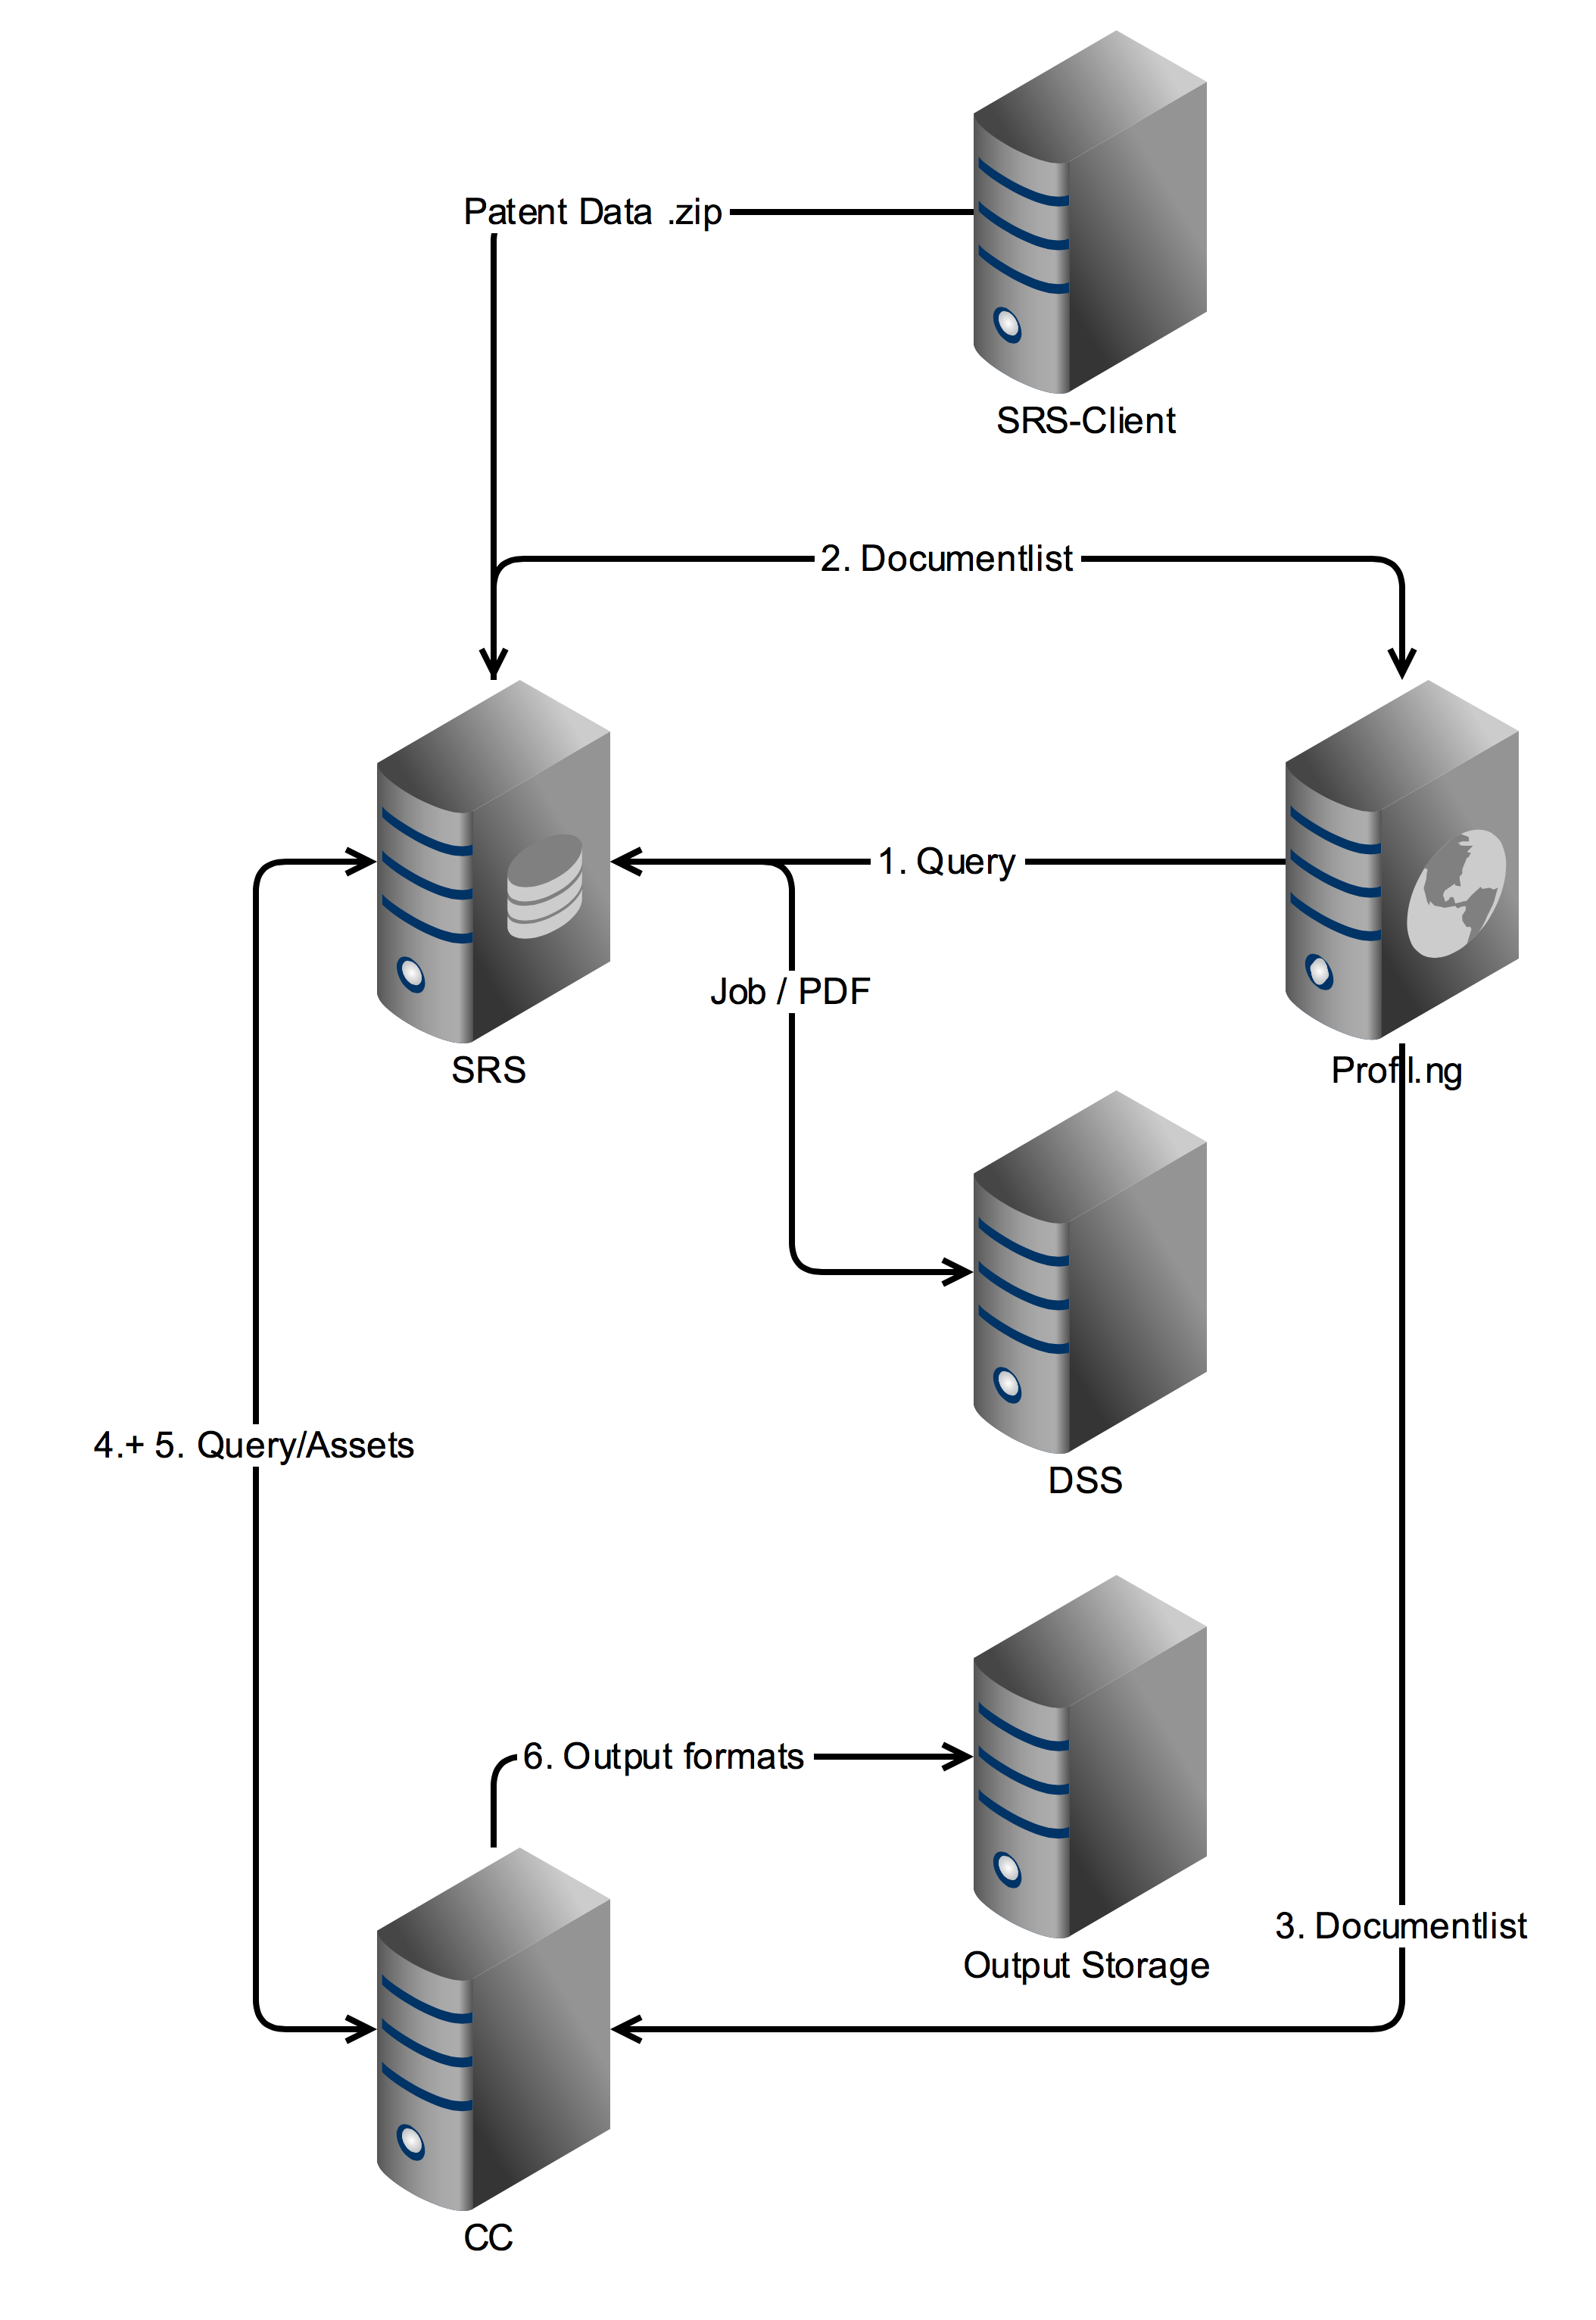
\includegraphics[width=0.9\textwidth]{gfx/dataflow-2.pdf}
  \caption{DEPAROM.NG Systemübersicht}
  \label{fig:DNGOverview}
\end{figure}

Die \autoref{fig:DNGOverview}, Seite \pageref{fig:DNGOverview} zeigt schematisch
das Zusammenspiel der verschiedenen Webdienste im DEPAROM.NG-Ökosystem.
Patentdaten werden als .zip-Dateien vom SRS-Client an den Simple Reference Store
übermittelt. Dieser verarbeitet die Patentdaten und speichert sie in
normalisierter Form ab. Wo notwendig, fordert der SRS beim DEPAROM Satz Service
(DSS) die Erstellung von Patentschriften im PDF-Format an.

Für die Produktion der Kundendatenträger sendet Profil.NG (PNG) eine Suchanfrage
an den SRS (1.). Dieser antwortet mit einer Dokumentliste, welche die
Dokument-IDs der gefundenen Patentdokumente enthält (2.). Anhand der
Dokumentliste erstellt PNG einen Job beim Collection Creator (3.), welcher die
notwendigen Artefakte zusammenträgt (4.+5.) und in einer Verzeichnisstruktur auf
dem Auslieferungsserver schreibt (6.), die dann auf einem Datenträger an den
Kunden übergeben werden.

\subsection{Simple Reference Store (SRS)}
\label{ch:fachlichesUmfeld:Teilsysteme:SRS}

Der sogenannte Simple Reference Store bildet den zentralen Datenspeicher von
DEPAROM.NG. Hier werden die Daten zu jedem Patentdokument gespeichert. Hierzu
gehören sowohl die originalen Dateien, wie sie von den jeweiligen Patentämtern
bezogen wurden, als auch normalisierte Daten im JSON und XML-Format. Das
normalisierte Format wird MTC-Format genannt. In \autoref{fig:SRSImport}, Seite
\pageref{fig:SRSImport} ist schematisch  der Datenstrom und die beteiligten
Softwarekomponenten aufgezeigt. Nachdem die Daten aus dem Patent-XML nach JSON
überführt wurden, werden auch die übrigen Artefakte (Zeichnungen, Faksimile)
extrahiert und auf einem Dateiserver abgelegt. SRS stellt auch diese Bild- und
PDF-Dateien bereit. Der Zugriff erfolgt über eine REST-Schnittstelle. Die
JSON-Formate werden in Elasticsearch gespeichert, indiziert und suchbar gemacht.

\begin{figure}[h]
  \includegraphics[width=0.9\textwidth]{gfx/srs-import.pdf}
  \caption{Datenstrom bei SRS-Import}
  \label{fig:SRSImport}
\end{figure}

SRS stellt auch eine Schnittstelle für Suchanfragen bereit, welche
Patentdokumente in konfigurierbaren Formaten und Detailgraden zurückliefert.

\subsection{DEPAROM Satz Service (DSS)}
\label{ch:fachlichesUmfeld:Teilsysteme:DSS}

Ein wichtiger Bestandteil der Patentinformationslieferungen aus DEPAROM.NG sind
die vollständigen Patentschriften im PDF-Format. Unglücklicherweise werden diese
nicht immer von den Patentämtern in der notwendigen Qualität geliefert. In
diesem Falle müssen die PDF-Dateien aus dem XML und den Bilddateien unter
Verwendung von XSL-FO erstellt werden. Der DSS übernimmt diese Aufgabe.

\subsection{DEPAROM Collection Creator (DCC)}
\label{ch:fachlichesUmfeld:Teilsysteme:DCC}

Der Dienst produziert Ausgabeformate, welche an Kunden für bestimmte
Dienstleistungen ausgeliefert werden. Derzeit produziert der DCC das für den
DEPAROM-Rechercheclient notwendige DVD-Format. Als Eingabedaten akzeptiert der
DCC Dokumentnummerlisten, anhand derer der Dienst die Patentdokumente
identifizieren kann, die in ein Ausgabeformat exportiert werden sollen.

\subsection{Profil.NG (PNG)}
\label{ch:fachlichesUmfeld:Teilsysteme:PNG}

Die Anwendung zur Steuerung des wöchentlichen Produktionsprozesses für den
Patentinformationsdienst DEPAROM Profil. PNG ist Gegenstand dieser
Bachelorarbeit. Sie soll die Operatoren befähigen, die
Patentinformationslieferungen zu produzieren und Abrechnungsdaten für die
Buchhaltung und Rechnungstellung zu generieren.
